\documentclass[conference]{IEEEtran}
\IEEEoverridecommandlockouts
% The preceding line is only needed to identify funding in the first footnote. If that is unneeded, please comment it out.
\usepackage{cite}
\usepackage{amsmath,amssymb,amsfonts}
\usepackage{algorithmic}
\usepackage{graphicx}
\usepackage{textcomp}
\usepackage{xcolor}
\usepackage{hyperref}
\usepackage{amsmath}
\usepackage{amssymb}

\newcommand{\rom}[1]{\uppercase\expandafter{\romannumeral #1\relax}}

\DeclareMathOperator*{\argmin}{arg\,min}

\def\BibTeX{{\rm B\kern-.05em{\sc i\kern-.025em b}\kern-.08em
    T\kern-.1667em\lower.7ex\hbox{E}\kern-.125emX}}
\begin{document}

\title{Assignment 1: a mathematical essay on logistic regression\\}


\author{\IEEEauthorblockN{Gautham Govind A}
\IEEEauthorblockA{\textit{Dept. of Electrical Engineering}\\
\textit{Indian Institute of Technology Madras} \\}
\textit{ee19b022@smail.iitm.ac.in}

}

\maketitle

\begin{abstract}
The objective of this assignment is to explore the mathematical formalism behind logistic regression and then to use it in a real-life application. In this assignment, as a real-life application, logistic regression is used to formally identify the factors which could have been used to  predict the chance of survival of an individual in the historical sinking of The Titanic. Data visualization, cleaning and modelling is done using Python. The analysis enables us to arrive at the conclusion that although luck played a major role in predicting survival, other factors like socioeconomic status and gender does indeed have an impact on the chance of survival. 
\end{abstract}

\begin{IEEEkeywords}
logistic regression, python, visualization, predictive modelling
\end{IEEEkeywords}

\section{Introduction}

The sinking of Titanic is one of the most tragic incidents in the history of humanity. On April 15, 1912, during her maiden voyage, the widely considered “unsinkable” RMS Titanic sank after colliding with an iceberg, resulting in the death of 1502 out of the total 2224 individuals (including passengers and the crew). Although there definitely was some element of luck involved in determining who survived and who did not, it is necessary to examine if any other factors( such as socioeconomic status) played a role in determining the survival of an individual. This can help in bringing out involuntary biases which may play a role in imposing disadvantages on certain sections of the society.

In this assignment, the goal is to make use of logistic regression to tackle the above mentioned problem. Logistic regression is a popular mathematical model for estimating how a binary variable is influenced by a variety of known factors. By performing logistic regression analysis, we will be able to get an idea of how each feature influences the target variable. This model can then be used for predicting the target variable from the known factors for cases in which the actual value of the target variable is unknown.

In this particular problem setting, the goal is to make use of a logistic regression model for the particular case of predicting whether an individual will survive the sinking of Titanic, provided we know certain characteristics of the individual, including but not limited to socioeconomic status and gender. By making use of data for which we know if an individual survived or not, we then build a model for the data for which we do not know this. The accuracy of the model can then be used to assess how good the identified relationships are.

Section \rom{2} gives an overview of the various techniques used for data cleaning, feature engineering and an initial exploratory analysis. A lot of insights can be gained just by making qualitative observations from the given data. Section \rom{3} gives a short description of the mathematical formalism behind logistic regression. Section \rom{4} sates the various results that are obtained by applying logistic regression in this particular case. Section \rom{5} gives a summary of the major conclusions drawn from the analysis.


\section{Exploratory Data Analysis}

In this section, we describe the process of data cleaning, feature engineering and data visualization.

\subsection{Data Cleaning}

We are given two datasets: a training dataset and a test dataset. The training dataset consists of 891 rows and 11 columns, whereas the test dataset consists of 418 rows and 10 columns. A brief overview of the training dataset is presented in Figure \ref{df_train_initial_info} and of the test dataset is presented in Figure \ref{df_test_initial_info}. We see that we know the ground truth values for whether the individual survived or not in the training dataset whereas we do not know this for the test dataset. We will keep the test dataset aside and use it only after we have completed building the model.

\begin{figure}[tbh]
\centering
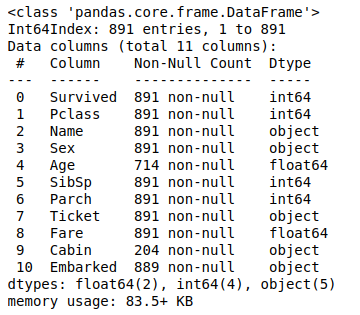
\includegraphics[scale = 0.45]{df_train_initial_info.png}
\caption{Summary of the training dataset}
\label{df_train_initial_info}
\end{figure}

\begin{figure}[tbh]
\centering
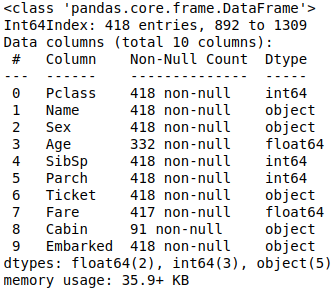
\includegraphics[scale = 0.45]{df_test_initial_info.png}
\caption{Summary of the test dataset}
\label{df_test_initial_info}
\end{figure}

Our next task is to account for the missing values in the dataset. We see that there are missing values in three columns: "Age", "Cabin" and "Embarked". Each column is dealt with separately and the procedure is described below.

The values in the column "Age" are plotted in a boxplot in Figure \ref{age_dist}. From the plot, it can be seen that the distribution \textbf{is skewed to the right.} In such scenarios, it is better to impute the missing values \textbf{using median as compared to mean.} Hence the missing values are replaced with the computed median, which happens to be 28. 

We see that we only have \textbf{202 non-null values for column "Cabin" out of the total 891, which is merely 22.67\%.} Since this is so low, we drop this column for predictive modelling. This is further supported by the fact that most of the datapoints in the test set also  do not have cabin values. However, we will use the available values to see if there is any correlation between cabin number and chance of survival.

Finally, for the column "Embarked" we have only 2 missing values. Since this is just 2 datapoints, we drop these rows. After handling the missing values, we end up with a dataset which is summarized by Figure \ref{df_train_final_info}.

We also note that the feature "Fare" has a missing value in the test set, but not in the training set. We perform mean imputing for this feature in the test set.



\begin{figure}[tbh]
\centering
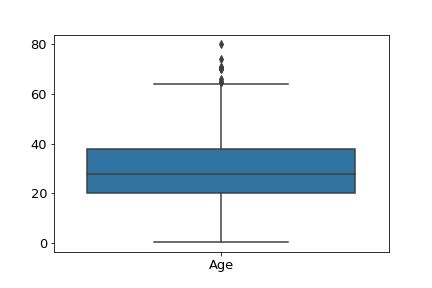
\includegraphics[scale = 0.55]{age_dist.png}
\caption{Distribution of age}
\label{age_dist}
\end{figure}

\begin{figure}[tbh]
\centering
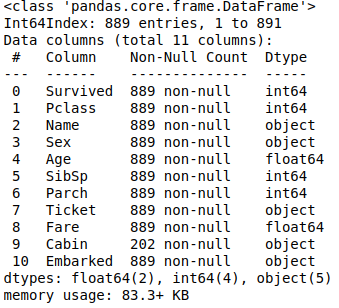
\includegraphics[scale = 0.55]{df_train_final_info.png}
\caption{Summary of the processed training dataset}
\label{df_train_final_info}
\end{figure}

\subsection{Data Visualization/ Qualitative Analysis}

To get a qualitative picture, we make plots of relevant features against the survival rate, which is the number of individuals who survived divided by the total number of individuals.

First, we make a barplot of passenger class, given by the column "Pclass". We obtain the plot given in Figure \ref{class_plot}. From the plot, it is evident that a higher fraction of passengers belonging to a higher passenger class survived as compared to passengers belonging to a lower passenger class. This could be \textbf{ due to the fact that higher class tickets were often taken by people who were economically and socially privileged thereby giving them an advantage over the lesser privileged sections in times of such crises.} This also reflects an inherent bias present in the society.

\begin{figure}[tbh]
\centering
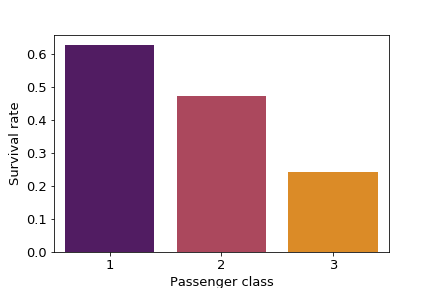
\includegraphics[scale = 0.55]{class_plot.png}
\caption{Survival rate v/s Passenger class}
\label{class_plot}
\end{figure}

Next, we make a barplot of gender, given by the column "Sex". We obtain the plot given in Figure \ref{sex_plot}. From the plot, it is evident that the \textbf{survival rate is higher for females as compared to males.} This could be because of the social norm of the time, which stipulated giving preference to women and children during times of disasters.

\begin{figure}[tbh]
\centering
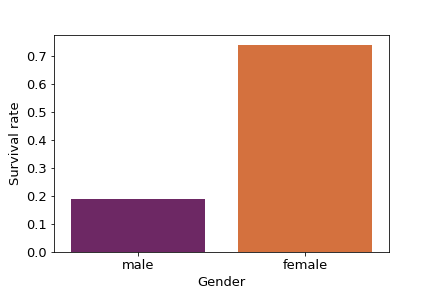
\includegraphics[scale = 0.55]{sex_plot.png}
\caption{Survival rate v/s Gender}
\label{sex_plot}
\end{figure}

Next, we make a kdeplot (kernel density estimate plot) of age, given by the column "Age". We obtain the plot given in Figure \ref{age_plot}. From the plot, we make two observations:

\begin{itemize}
    \item There was a \textbf{greater chance for children to survive.} Again, this could be because priority was given to women and children during evacuation.
    \item \textbf{A greater fraction of people in the age group 20-40 did not survive} compared to other age groups; this could be because they stayed back to aid younger and older individuals during evacuation.
\end{itemize}

\begin{figure}[tbh]
\centering
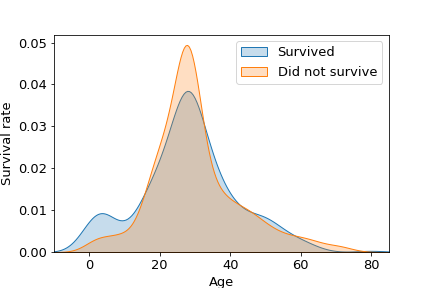
\includegraphics[scale = 0.55]{Agevssurvival.png}
\caption{Survival rate v/s Age}
\label{age_plot}
\end{figure}

Next, we make a kdeplot (kernel density estimate plot) of fare, given by the column "Fare". We obtain the plot given in Figure \ref{farevssurvival}. It can be seen that, in general, \textbf{people who paid a higher fare had a higher chance for survival.} This could again be associated with higher social and economic status and the associated privilege, as generally only the richer sections can afford to pay a higher fare.

\begin{figure}[tbh]
\centering
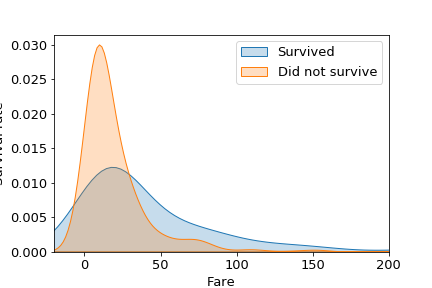
\includegraphics[scale = 0.55]{farevssurvival.png}
\caption{Survival rate v/s Fare}
\label{farevssurvival}
\end{figure}

Next, we explore if there is any relationship between cabin and survival rate. Since considering each cabin separately is impractical, we consider only the cabin group, which is given by the alphabet preceding the number. Note that we do this only for the datapoints for which the cabin information is available. Rest of the datapoints are assigned the cabin group "U". We obtain the plot given in Figure \ref{cabin_group_plot}. Due to the limited data available, it is not possible to make conclusive statements regarding the impact of cabin group on survival rate. However, if more data is available, it might be possible to correlate the cabin group with survival rate as we intuitively expect certain cabin groups to have more access to lifeboats and other such similar factors.

\begin{figure}[tbh]
\centering
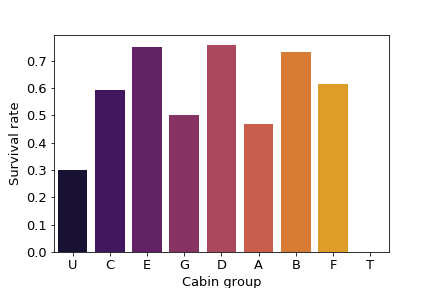
\includegraphics[scale = 0.55]{cabin_group_plot.png}
\caption{Survival rate v/s Cabin group}
\label{cabin_group_plot}
\end{figure}

\subsection{Feature Extraction}

In this section, we look at manipulating some of the existing features so as to make them more useful.

We do not expect the name of an individual to directly have any influence on his/her survival chance. However, \textbf{the honorifics associated with the name might have an impact on survival chance.} Hence, we extract the honorifics and store them in a separate column titled "title". We expect this feature to capture the socioeconomic status of an individual.

The categorical features we have now are "Pclass", "Sex", "Embarked" and "title". Of these, "Pclass" which denotes the passenger class has a numbering by default; as we have seen before, higher the class of the passenger, higher is the chance of survival. Hence, we maintain the existing numerical ordering for this feature.

For the other features, we implement one-hot encoding. We cannot employ ordinal ordering as this would enforce an ordering of classes which does not naturally exist. Although in some applications doing one-hot encoding would blow up the number of features, in this case, since we only have a limited number of features, one-hot encoding is feasible. After performing one-hot encoding, we end up with the dataset summarized in Figure \ref{df_feat_info}.

\begin{figure}[tbh]
\centering
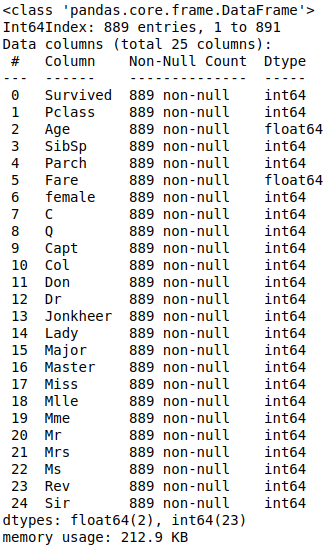
\includegraphics[scale = 0.45]{df_feat_info.png}
\caption{Summary of dataset after feature extraction}
\label{df_feat_info}
\end{figure}



\section{Model: Logistic Regression}

In this section, we will give a brief overview of the mathematical formalism behind the logistic regression model. 

Logistic Regression (also called Logit Regression) is a model commonly used to estimate the probability that an instance belongs to a particular class out of K given classes. The most common version is the one with K = 2, in which case the classification is binary. If the estimated probability is greater than 50\%, then the model predicts that the instance belongs to that class (called the positive class, labeled “1”), and otherwise it predicts that it does not (i.e., it belongs to the negative class, labeled “0”).

Logistic Regression is a linear model for classification, which means the decision
surfaces are linear functions of the input vector x. The simplest case is to model $y(\mathbf{x}) = \mathbf{w^Tx} + w_0$ so that y is a real number. But for a classification problem, we seek to
obtain probabilities that lie in (0,1) range. Hence, we apply a
non-linear function $f ()$ such that $$y(\mathbf{x}) = f(\mathbf{w^Tx }+ w_0 )$$ returns the posterior probabilities. Decision surfaces correspond to $y(x) = \textrm{constant}$ , which implies $\mathbf{w^Tx} + w_0 = \textrm{constant}$ for one to one f, which makes the decision boundary linear. An example of such a decision boundary is given in Figure \ref{decision-boundary}.

\begin{figure}[tbh]
\centering
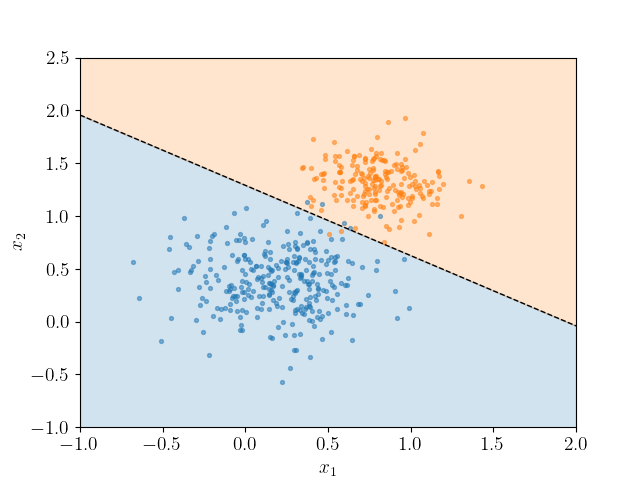
\includegraphics[scale = 0.50]{decision-boundary.png}
\caption{Linear decision boundary of logistic regression}
\label{decision-boundary}
\end{figure}

The non-linear function $f ()$ used in logistic regression is a sigmoid function (also known as logistic function) that outputs a number between 0 and 1: $$ \sigma(u) = \frac{1}{1 + e^{-u}} $$ $$ \hat{p} = \sigma(\mathbf{w^Tx} + w_0) $$

The estimated probabilities can easily be converted into a binary classifier by predicting

$$   \hat{y}= 
\begin{cases}
    C1,& \textrm{if } \hat{p} < \textrm{Threshold}\\
    C2, & \text{otherwise}
\end{cases} $$



where $C 1$ and $C 2$ are the two classes. The threshold is usually
set to 0.5.

\subsection*{Parameter Estimation}

The parameters can be estimated using Maximum Likelihood Estimation (MLE). Let the number of data points be $M$ and $i$ be an integer such that $1 \leq i \leq M$; $i$ is used to index a datapoint in the dataset. Let $y_i$ denote the ground truth corresponding to datapoint $x_i$. Then the Likelihood, given by $L(\mathbf{w})$ is:


\begin{align*}
    L(\mathbf{w}) &= P(y_1, y_2, ..., y_m|x_1, x_2, ..., x_m) \\
 &= \Pi_{i = 1}^{M} P(Y_i = y_i|X_i x_i, \mathbf{w}) \\
 &= \Pi_{i = 1}^{M}\sigma(y_i\mathbf{w^T}x_i)  \\
 \log{ L(\mathbf{w})} &= \sum_{i = 1}^{M}\log{\sigma(y_i\mathbf{w^T}x_i)}
\end{align*}

We could maximise log-likelihood or minimise negative log-likelihood to estimate the parameters. Or equivalently, minimise Empirical Logistic Loss function, $\hat{R}(\mathbf{w})$ defined as:
$$ \hat{R}(\mathbf{w}) \triangleq -\log{L(\mathbf{w})} = \sum_{i=1}^{M}\log{(1 + \textrm{exp}(-y_i\mathbf{w^T}x_i))}$$
      
The goal is to minimize $\hat{R}(\mathbf{w})$; however there exists no closed form solution. So we make use of Gradient Descent. The steps involved in the gradient descent algorithm for logistic regression are briefly outlined below:

\begin{itemize}
    \item Initialize $\mathbf{w_t} = \mathbf{w_0}$ randomly.
    \item Repeat till convergence:
    \begin{align*}
        \mathbf{w_{t+1}} &= \mathbf{w_t} - \eta \nabla{ \hat{R}(\mathbf{w_t})} \\
        &= \mathbf{w_t} - \eta \sum_{i = 1}^{M}\sigma({-y_i\mathbf{w_t^T}x_i})(-y_ix_i)
    \end{align*}
\end{itemize}

where $\eta$ is the learning rate and $t$ is the iteration number.

\subsection*{Regularised Logistic Regression}

In order for the model to generalise well and to prevent over-fitting, a penalty function could be added to the loss function. We choose the $L2$ norm and hence this is termed Ridge regression. For the $L2$ norm penalty function, the empirical loss function becomes:

$$ \hat{R}(\mathbf{w}) = \sum_{i=1}^{M}\log{(1 + \textrm{exp}(-y_i\mathbf{w^T}x_i))} + \frac{\lambda}{2}||\mathbf{w}||^2 $$

where $\lambda$ denotes the regularization parameter, which is treated as a hyper-parameter. The modified expression of $\hat{R}(\mathbf{w})$ is then used for performing gradient descent.

\section{Modelling }

In this section, we discuss the application of the logistic regression model to our problem. 

The logistic regression is trained on the training set using gradient descent. The training process is abstracted out through the sklearn library. The only \textbf{hyper-parameter present in the model is $\lambda$,} which is the \textbf{regularization parameter.} The \textbf{best value of $\lambda$ is found out using cross-validation,} which involves breaking up the training data into multiple sets, evaluating different values of $\lambda$ and choosing the most suitable value.

The predictive model for a classification problem can be evaluated using multiple metrics. A short description of the most commonly used metrics is given below:

\begin{itemize}
    \item \textbf{Accuracy:}
    Accuracy is simply the \textbf{ratio of number of correct predictions to total number of predictions.} Although this seems like a very good metric intuitively, accuracy fails on classification problems with a skewed class distribution because of the intuitions developed by practitioners on datasets with an equal class distribution.
    \item \textbf{Precision:}
    Precision is the \textbf{ratio of true positives to the total positive predictions.} Precision is typically used when the cost of false positive is high. For instance, email spam detection.
    \item \textbf{Recall:}
    Precision is the \textbf{ratio of true positives to the total positive ground truths.} Recall is typically used when the cost of false negative is high. For instance, in fraud detection or sick patient detection.
    \item \textbf{F1-score:}
    F1-score is simply a \textbf{harmonic average of precision and recall.} F1 Score is typically used if we need to seek a balance between Precision and Recall and there is an uneven class distribution.
    
    
\end{itemize}

The confusion matrix for the training set is shown in Figure \ref{ConfusionMatrix}. The values for the evaluation metrics are given in Table \ref{metric_table}. From this analysis, it is clear that we can \textbf{predict the survival chance of an individual to a reasonable extent from the parameters used.} This indicates that there indeed exists some correlation between survival chance and factors like socioeconomic status and gender. Predictions were also made for the entries in the test set. However, the quality of predictions could not be evaluated as labels were not available.

\begin{figure}[tbh]
\centering
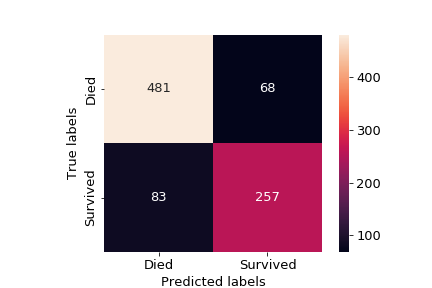
\includegraphics[scale = 0.55]{ConfusionMatrix.png}
\caption{Confusion matrix for the training set}
\label{ConfusionMatrix}
\end{figure}

\begin{table}
\begin{center}

\caption{Evaluation of Logistic Regression model}

\begin{tabular}{| c| c| }
 \hline
 Metric & Score \\
 \hline
 \hline
 Accuracy & 0.831 \\ 
 \hline
 Precision & 0.791 \\   
 \hline
 Recall & 0.759 \\
 \hline
 F1 Score & 0.775 \\
 \hline

\end{tabular}

\label{metric_table}
\end{center}

\end{table}

ROC curve is another common tool used with binary classifiers. A Receiver Operating Characteristic curve, or ROC curve, is a graphical plot that illustrates the diagnostic ability of a binary classifier system as its discrimination threshold is varied. The ROC curve is created by plotting the true positive rate (TPR) against the false positive rate (FPR) at various threshold settings. The ROC curve for the logistic regression model is given in Figure \ref{Rocauccurve}.

\begin{figure}[tbh]
\centering
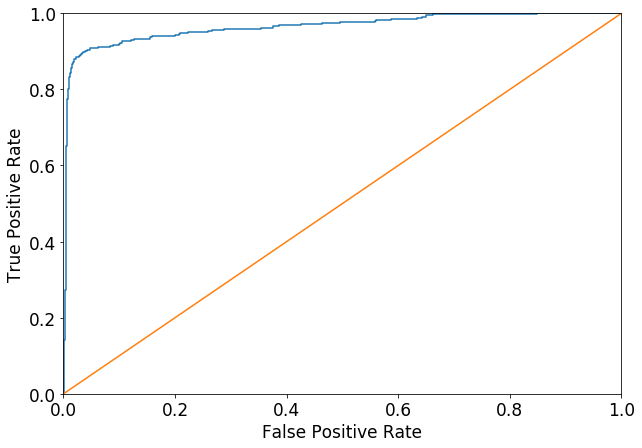
\includegraphics[scale = 0.55]{Rocauccurve.png}
\caption{ROC curve}
\label{Rocauccurve}
\end{figure}

The dotted line represents the ROC curve of a purely random classifier; a good classifier stays as far away from that line as possible (toward the top-left corner). One way to compare classifiers is to measure the area under the curve (AUC). A perfect classifier will have a ROC AUC equal to 1, whereas a purely random classifier will have a ROC AUC equal to 0.5. \textbf{The area under the ROC curve of our logistic regression classifier is 0.876.}

\section{Conclusions}

From the logistic regression model, we were able to arrive at the conclusion that although luck did play a role in determining who survived and who did not, it also depended on a variety of other factors. In particular, it was found that \textbf{passengers in first class, women, children and people who paid a higher fare were all more likely to survive.} We were also able to make predictions of whether an individual will survive or not for cases where the ground truth was unknown. This analysis helps bring out biases which society as a whole may voluntarily or involuntarily hold against sections of the population. Closely reflecting on such analyses and focusing on their implications can help better everyone's lives.



\section{Avenues for further research}

Although logistic regression is a powerful model, it is only a linear model. Making use of non-linear models, either by considering non-linear models or by using kernels for introducing non-linearity is an avenue worth exploring. Collecting more features (like proximity to lifeboats) could also help improve modelling.




\nocite{*} % Print all references regardless of whether they were cited in the poster or not
\bibliographystyle{ieeetr}
\bibliography{sample} % Use the example bibliography file sample.bib


\end{document}

